\section{Energy Efficiency}

	We tried to measure the board's current consumption as in \cite{tdt4258-1} with SLDDD's \textit{splash screen} running, using a FLUKE 177 TRUE RMS MULTIMETER that was located in room itv442.
 	Measuring the current across \texttt{VDDCORE} proved to be unfeasible as the STK1000's did not seem to progress past the initial completely white screen when turned on while the measuring equipment was connected to the \texttt{VDDCORE} pins.

\begin{table}[h]
	\centering
    \begin{tabular}{|l|l|}
    \hline
    Pins & Measurement \\ \hline
    \texttt{AVDDUSB} (1,2) & 0.28mA \\ \hline
    \texttt{AVDDPL} (3,4) & 4.01mA \\ \hline
    \texttt{AVDDOSC} (5,6) & 0.01mA \\ \hline
    \texttt{VDDCORE} (7,8) & N/A \\ \hline
    \texttt{VDDIO} (9,10) & 2.55mA \\ \hline
    \end{tabular}
    \caption{Measurements of current consumption taken on the STK1000.}
    \label{table-currentmeasurements}
\end{table}
	
	Other than that, the solution does not make use of interrupts.

\section{Testing}
\subsection{Basic functionality tests}
	\subsubsection{LED \& button driver test}
		\begin{description}
			\item[Description] \hfill \\
				This test is designed to assertain whether the LED and button drivers function as intended.
			\item[Prerequisites] \hfill
				\begin{itemize}
					\item{a driver for the STK1000's LEDs.}
					\item{a driver for the STK1000's buttons.}
					\item{a working installation of Linux running on the STK1000.}
					\item{The LED driver must be able to parse the data produced by reading the buttons' state through the button driver.}
				\end{itemize}
			\item[Procedure] \hfill
				\begin{enumerate}
					\item{Load the LED \& button drivers using \texttt{insmod} and \texttt{mknod}.}
					\item{enter \texttt{cat /dev/buttons > /dev/leds} into the console.}
				\end{enumerate}
			\item[Expected results] \hfill \\
				When \texttt{SWn} is held down \texttt{LEDn} should light up.
				\\$n \in [0,7]$
		\end{description}	

\subsection{Game test suite}

	\subsubsection{Unit tests}

    Parts of the code base are covered with unit tests, using a simple but nice unit test framework called muunit.
    These unit tests have been particularly helpful in finding platform specific bugs.
        

	\subsubsection{Fontenizening, the testening}
		\begin{description}
	\item[Description] \hfill \\
		This test is meant to verify the functionality of the font engine.
	\item[Prerequisites] \hfill
		\begin{itemize}
			\item{A possibly working font rendering engine or similar device.}
			\item{Text you want to render.}
		\end{itemize}
	\item[Procedure] \hfill
		\begin{enumerate}
			\item{Feed the text to the font rendering engine.}
		\end{enumerate}
	\item[Expected results] \hfill \\
		Given text is rendered on the screen.
	\item[Actual results] \hfill \\
		See figure~\ref{img-fontengine}.
	\begin{figure}[h!]
			\centering
			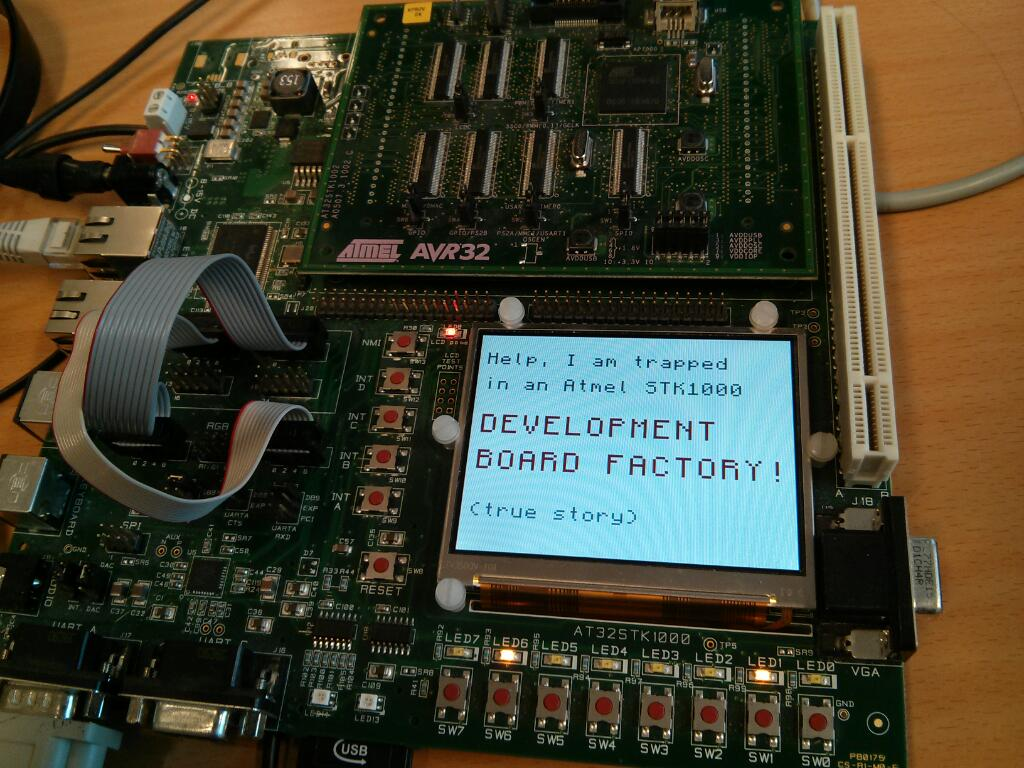
\includegraphics[width=4in]{{images/fontengine-test.jpg}}
			\caption{Actual result obtained from conducting font engine tests.}
			\label{img-fontengine}
	\end{figure}
	
\end{description}

	\subsubsection{Evaluating the efficiency of functions}
		Select functions print their runtime/TTC (time to completion) to the console, allowing an evaluation to be made regarding their efficiency.
		This facilitates the evaluation of changes made to functions: if a change in the function results in an increase in its runtime, the change did not contribute to increased efficiency.
        This kind of profiling is essential when making a program with real-time requirements, such as a rhythm music game, as it allows for easy detection and possible elimination of inefficiencies in the code.
		This particular technique using print statements and time calculation is a kind of profiling\footnote{\url{http://en.wikipedia.org/wiki/Profiling\_(computer\_programming)}} dubbed ``ghetto profiling'' by one of the authors. 
        Ghetto profiling was chosen over profiling with a fully featured profiler like \texttt{gprof} when running on the STK1000, because getting gprof to run nicely on the STK1000 is hard.

\subsection{Gameplay}
	\begin{description}
		\item[Description] \hfill \\
			Video games are a recreational activity.
			That means people play them in their spare time.
			Who would want to spend their spare time doing something that's not enjoyable?
			This test is designed to uncover what parts of the video game that are enjoyable and what parts are less enjoyable.
		\item[Prerequisites] \hfill
			\begin{itemize}
				\item{A working build of the solution.}
				\item{One or more live subjects.}
			\end{itemize}
		\item[Procedure] \hfill
			\begin{enumerate}
				\item{Introduce the subject to the solution.}
				\item{Allow the subject to attempt to interface with the solution.}
				\item{Wait.}
				\item{Collect feedback from subject.}
			\end{enumerate}
		\item[Expected results] \hfill \\
			Feedback from the participants.
		\item[Actual results] \hfill \\
			This test was run with four subjects.
			Subjects 1-3 reported that the game occasionally lagged, resulting in a ``loss of combo''.
			In addition they commented on the speed with which the hexagons moved across the screen, saying it ``might be a bit fast''.
			They also noted that if a button is held down then all steps in its lane are automatic hits (usually a perfect or great).

			Subject 4 reported feeling a sharp pain in his fingertips once gameplay was concluded.
	\end{description}


\section{Discussion}

On the topic of energy efficiency: the presented solution game does not employ some of the common tricks for energy savings, such as using interrupts for handling button input.
However, the difference between an interrupt-based solution and an active polling one on the STK1000 has previously been suggested to be near-negligible\cite{tdt4258-1}.

	Due to feedback from test subjects during the early stages of development we decided to not implement two-player mode, as having two people trying to fit eight fingers in total on the STK1000's buttons was reported to be ``unpleasant''.
	
	The game occasionally stutters while in-song, to the frustration of the players. This is most likely because of cache misses, page faults and similar things when reading a large audio file from memory.
    Although a stutter here and there is not a great thing for the user experience, care was taken to make sure the game arrows never fall out of sync with the music, even through lags and glitches.
